% Updated by Michael Gertz, April 2021
%%%%%%%%%%%%%%%%%%%%%%%%%%%%

\documentclass{beamer}
%\usepackage[ngerman]{babel}
\usepackage[utf8]{inputenc}
\usepackage{multirow}

\usepackage{color}
\usepackage{graphicx}
\usepackage{fancybox}
\usepackage{comment}
\usepackage{algorithm}
\usepackage{algorithmic}
\setbeamertemplate{theorems}[numbered]
\renewcommand{\algorithmicrequire}{\textbf{Input:}}
\renewcommand{\algorithmicensure}{\textbf{Output:}}

\usepackage{natbib}


\usepackage{beamerthemesplit}
\usetheme[compress]{Heidelberg}
\definecolor{unirot}{rgb}{0.5976525,0,0}
\usecolortheme[named=unirot]{structure}


\title[Dense Retrieval with Entity Views]{Dense Retrieval with Entity Views}
\subtitle{Seminar ``Modern Infomation Retrieval'', Summer 2023}
%\subtitle{Subtitle}
\author[Johannes Sindlinger]{Johannes Gabriel Sindlinger}
\date{June 15, 2023}
\institute[Uni HD]{
Heidelberg University\\
Prof. Dr. Michael Gertz / Ashish Chouhan\\
Institute of Computer Science\\
Database Systems Research Group\\
\color{unirot}{johannes.sindlinger@stud.uni-heidelberg.de}}

%---------------------------------------%
%---------- RECURRING OUTLINE ----------%
% have this if you'd like a recurring outline
\AtBeginSection[]  % "Beamer, do the following at the start of every section"
{
\begin{frame}<beamer> 
\frametitle{Outline} % make a frame titled "Outline"
\tableofcontents[currentsection,hideallsubsections]  % show TOC and highlight current section
\end{frame}
}
%----------------------------------------

\begin{document}
\frame[plain]{\titlepage}

%========================================
%========================================

\frame{
\frametitle{Relevance of Paper}

{\color{unirot}Authors:} 
  \begin{itemize}
    \item Hai Dang Tran (Max Planck Institute for Informatics)
    \item Andrew Yates (University of Amsterdam)\\[5pt]
  \end{itemize}
{\color{unirot}Publication Date:} 17 October 2022 \\[5pt]
{\color{unirot}Publication Conference:} CIKM '22: Proceedings of the 31st ACM International Conference on Information \& Knowledge Management\\[25pt]

{\color{unirot}Citations:} 0 \\[5pt]
{\color{unirot}Downloads on ACM\footnote{last retrieved June 3, 2023}:} 316


}

\frame{\frametitle{Outline}\tableofcontents[hideallsubsections]}

\section[Motivation]{What's the issue? -- Motivation}

\frame{
\frametitle{Introduction -- Bi-Encoder Model}
\begin{figure}
  \includegraphics[width=0.85\textwidth]{Grafiken/Dense_Retrieval_Overview.png} 
\end{figure}
}

\frame{
\frametitle{Motivation}
\begin{figure}
  \includegraphics[width=\textwidth]{Grafiken/Problem.png} 
\end{figure}
$\Rightarrow$ Language models do not fully capture information about real-world entities, especially for uncommon entities.
}

\frame{
\frametitle{Example}
\begin{figure}
  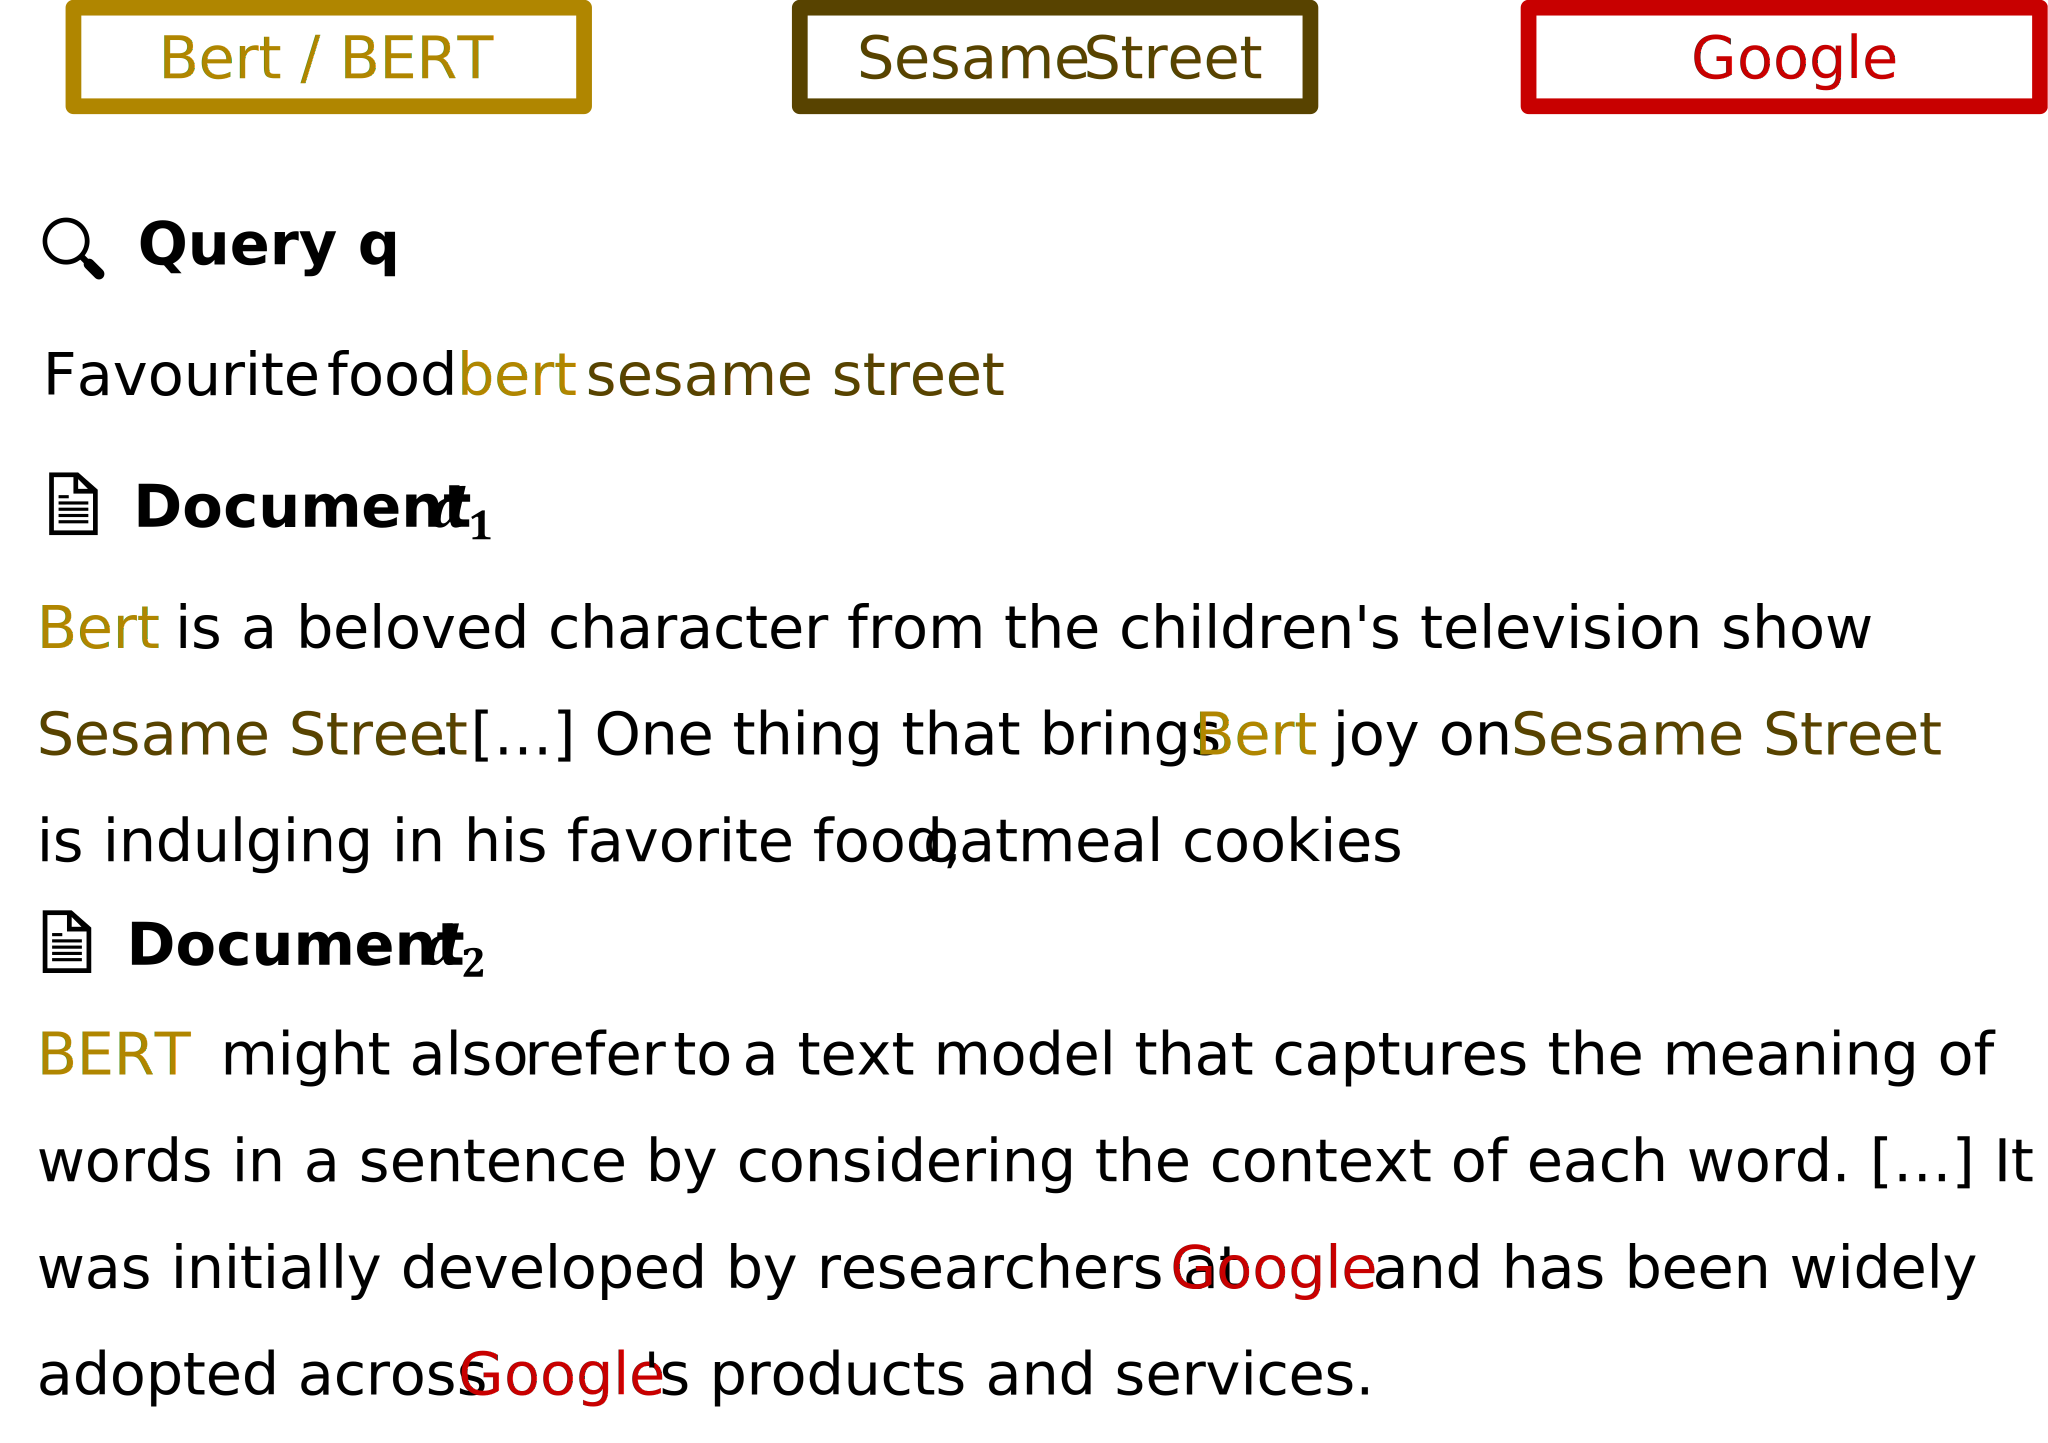
\includegraphics[width=\textwidth]{Grafiken/Example_3_Entities.png} 
\end{figure}
}


%---------------------------------------
%---------------------------------------
\section[Related Work]{What has been already there? – Related Work}

\frame{
\frametitle{Related Work}

{\color{unirot}Pre neural IR models:} Extending queries with entity descriptions or features (e.g. synonyms, relationships) \\[5pt]
{\color{unirot}Within neural IR models:}
\begin{itemize}
\item Interaction-based ranking methods (e.g. KNRM\footnote{\cite{knrm}, additionally applied to the approach of this paper})
\item Including entities within learning procedure (e.g. ERNIE\footnote{\cite{sun2020ernie}})
\end{itemize}
\vspace{5pt}
{\color{unirot}\textbf{What's new?}} Including entity representations \textbf{independently} of pre-trained language model.
}

%---------------------------------------
%---------------------------------------
\section[Methodology]{What‘s new? – Methodology}

\frame{
\frametitle{General Model}
\begin{figure}
  \includegraphics[width=\textwidth]{Grafiken/Main_Idea.png} 
\end{figure}
}

\frame{
\frametitle{Extracting Entities}
\begin{figure}
  \includegraphics[width=0.9\textwidth]{Grafiken/Extracting_Entities.png} 
\end{figure}
}


\frame{
\frametitle{Kernel Pooling Score -- KNRM}
{\color{unirot}\underline{Idea:}} Find documents where entities of documents and query have high similarity value using \underline{k}ernel-based \underline{n}eural \underline{r}anking \underline{m}odel. \\[5pt]
$\Rightarrow$ \textbf{Interaction-based} approach \\[10pt]
\begin{enumerate}
  \item Get entity interaction matrix between the set of entities within query $\mathbf{E}(q)$ and document $\mathbf{E}(d)$:
  \[T_{i,j} := sim(\mathbf{E}_i(q), \mathbf{E}_j(d))\]
  \item Build k kernels for each entity of q using radial basis function, which creates differentiable histograms around given $\mu$ and $\sigma^2$
  \item Calculate a pooled / summarized representation of kernels and apply final (learned) ranking layer on that.
\end{enumerate}
}


\frame{
\frametitle{Generating Embeddings -- Queries}
\begin{figure}
  \includegraphics[width=\textwidth]{Grafiken/Main_Idea_Query_Embeddings.png} 
\end{figure}
}

\frame{
\frametitle{Generating Embeddings -- Queries}
{\color{unirot}\underline{Idea:}} Combine all Entities within Query (since query is unknown in advance, keep this method for all approaches)
\begin{figure}
  \includegraphics[width=\textwidth]{Grafiken/Single_Entity_Representation.png} 
\end{figure}
}


\frame{
\frametitle{Generating Embeddings -- Documents}
\begin{figure}
  \includegraphics[width=\textwidth]{Grafiken/Main_Idea_Document_Embeddings.png} 
\end{figure}
}

\frame{
\frametitle{Generating Embeddings -- Documents}
\begin{itemize}
  \item Single Entity Representation (EVA\footnote{EVA $\widehat{=}$ \underline{E}ntity \underline{V}iews in Dense Retriev\underline{a}l} Single)
  \item Query-Aware Single Entity Representation (EVA Single-QA)
  \item Multiple Entity View Representation (EVA Multi)
\end{itemize}
\vspace{0.5cm}
$\Rightarrow$ Optionally for all models: Adding Kernel pooling score (i.e. KNRM)
}

\frame{
\frametitle{EVA Single}
{\color{unirot}\underline{Idea:}} Combine all Entities within Document / Passage \\[8pt]
$\Rightarrow$ Problem: No focus on query information, possibly including irrelevant entities
\begin{figure}
  \includegraphics[width=\textwidth]{Grafiken/QA_Single_Entity_Representation_Document.png} 
\end{figure}

}

\frame{
\frametitle{EVA Single-QA}
{\color{unirot}\underline{Assumption:}} Query is known before calculations \\[8pt]
{\color{unirot}\underline{Idea:}} Select only entities in document with high similarity to query entities \\[8pt]
\begin{figure}
  \includegraphics[width=\textwidth]{Grafiken/QA_Single_Entity_Representation.png} 
\end{figure}
$\Rightarrow$ Problem: Large latency, EVA Multi solves this issue
}

\frame{
\frametitle{EVA Multi / 1}
{\color{unirot}\underline{Idea:}} Different queries require different views on entities \\[5pt]
$\Rightarrow$ Build embeddings for clusters of entities within document.
\begin{figure}
  \includegraphics[width=0.95\textwidth]{Grafiken/Multiple_Entity_View_Representation.png} 
\end{figure}
}

\frame{
\frametitle{EVA Multi  / 2}
\textbf{Building clusters removes assumption knowing the query in advance.}\\
\[\text{\underline{Why?}}\]
Recall filtering algorithm for EVA Single-QA: For each entity in the query q at maximum one close entity of the document d is selected.
\begin{block}{}
  \centering
  $\Rightarrow |\text{Entities in q}| \geq |\text{Filtered embeddings of d}|$
\end{block}
Analyzing data: $>$ 99\% queries contain at maximum 2 entities.\\
\begin{center}
  $\Rightarrow$ Clusters of size 1 and 2 are enough, can be enumerated easily.
\end{center}
}


\section[Results]{What's the outcome? – Results
}

\frame{
\frametitle{Experimental Setup}
\begin{itemize}
  \item Training data: MS MARCO\footnote{\cite{nguyen2016ms}} (300,000 training samples, 7,127 test samples)
  \item Evaluation data: MS MARCO Dev, TREC Deep Learning (DL) Track 2019\footnote{\cite{trec_dl_2019}}, TREC DL 2020\footnote{\cite{trec_dl_2020}}, TREC DL HARD\footnote{\cite{dl_hard}}
  \item Evaluation metrics: nDCG@10, MRR@10, MAP@1000
\end{itemize}
}

\frame{
\frametitle{Results}
\begin{overprint}
\onslide<1>
\begin{figure}
  \includegraphics[width=\textwidth]{Grafiken/Results_all.png} 
\end{figure}
\onslide<2>
\begin{figure}
  \includegraphics[width=\textwidth]{Grafiken/Results_all_selected.png} 
\end{figure}
\end{overprint}
}


\frame{
\frametitle{Exemplary Results}
\begin{figure}
  \includegraphics[width=\textwidth]{Grafiken/Results.png} 
\end{figure}
}

\frame{
\frametitle{Takeaways}
\begin{overprint}
  \onslide<1>
  \begin{figure}
    \includegraphics[width=\textwidth]{Grafiken/Results2.png} 
  \end{figure}
  \onslide<2>
  \begin{figure}
    \includegraphics[width=\textwidth]{Grafiken/Results3.png} 
  \end{figure}
  \onslide<3>
  \begin{figure}
    \includegraphics[width=\textwidth]{Grafiken/Results4.png} 
  \end{figure}
  \onslide<4>
  \begin{figure}
    \includegraphics[width=\textwidth]{Grafiken/Results5.png} 
  \end{figure}
\end{overprint}
}

\frame{
\frametitle{Personal opinion}

\begin{columns}[t]
\begin{column}{.5\textwidth}
{\color{unirot}Likes}

\small
\begin{itemize}
  \item Adding entities outperform basic Bi-Encoder approach significantly
  \item Multi-View approach seems reasonable and increase efficiency as well effectiveness
  \item Interpretable intuition
\end{itemize}
\normalsize
\end{column}


\begin{column}{.5\textwidth}
{\color{unirot}Dislikes} 
\small
\begin{itemize}
  \item Focus on entities is irrelevant for many queries, i.e. 43.5\% of queries during training process are reported to have 0 entities.
  \item Only focusing on TAS BERT and ERNIE as Pre-trained language model.
\end{itemize}
\normalsize
\end{column}

\end{columns}

\vspace{0.4cm}

{\color{unirot}Possible Improvements}: Adding other attributes in addition to entities, e.g. metadata (geographical, time, etc.), keyword embeddings, ...
} % END OF FRAME


\frame{\frametitle{Questions}
\begin{figure}
\includegraphics[width=\textwidth]{Grafiken/example} 
\end{figure}
\vspace{-4cm}
\begin{center}
  \begin{LARGE}
    \textbf{Thanks for your attention!} \\
    Questions?
  \end{LARGE}
\end{center}
\vspace{2.5cm}
}

\appendix

\nocite{trec_dl_2020,johnson2019billion,heinzerling2021language,ceccarelli2013dexter,yamada2018wikipedia2vec}
  

\frame[allowframebreaks]{
\small
\frametitle{References}
\setbeamertemplate{bibliography item}[text]
\bibliographystyle{plainnat}
\bibliography{references.bib}
}

\section*{Appendix}


\frame[allowframebreaks]{
\frametitle{Calculating KNRM}
\begin{enumerate}
  \item Let $\mathbf{E}(q)$ be the set of entities within query q, $\mathbf{E}(d)$ the set of entities within document d. Then the entity interaction matrix is given as: 
  \[T_{i,j} := sim(\mathbf{E}_i(q), \mathbf{E}_j(d))\]
  \item Build k kernels using radial basis function, which creates differentiable histograms around given $\mu$ and $\sigma^2$
  \[ K_l(\mathbf{E}_i(q)) = \sum_{j=1}^{|\mathbf{E}(p)|}\exp\left(-\frac{(T_{i,j}-\mu_i)^2}{2\sigma_i^2}\right)\]
  \item Pool / Summarize the k results into a k-dimensional feature vector \[\overrightarrow{K(\mathbf{E}_i(q))} = [K_1(\mathbf{E}_i(q)), \ldots, K_k(\mathbf{E}_i(q))]\]
  \item Build kernel-pooled representation $\phi(T)$ by calculating log-sum for each query entity \[\phi(T) = \sum_{i=1}^{|\mathbf{E}(q)|} \log \overrightarrow{K(\mathbf{E}_i(q))}\]
  \item Get final kernel pooling score by applying a learned ranking layer \[ \mathbf{S}_{\text{kp}} = \tanh(w^T\phi(T) + b) \]
\end{enumerate}
}


\frame{
\frametitle{Definitions: Pretrained Language Model Representation}

\begin{definition}
  Given a query or passage as text $t$ the textual representation $\mathbf{R}_{text}(t)$ of $t$ is formed by passing t to a pre-trained language model (PLM), i.e. distilled TAS (\cite{distilbert2020}). So it yields:
  \[\mathbf{R}_{text}(t) = \text{PLM}_{\text{CLS}(t)}\]
\end{definition}

\begin{definition}
  Let $\mathbf{E}_{all}(q)$ be the set of all entities mentioned in query $q$. The query entity representation $\mathbf{R}_{all}(q)$ is then the average embedding of entities in $\mathbf{E}_{all}(q)$.
\end{definition}
}


\frame{
\frametitle{Definitions: Single Entity Representation}

\begin{definition}
  The query-independent passage entity representation $\mathbf{R}_{all}(p)$ is defined as the average embedding of entities in $\mathbf{E}_{all}(p)$.
\end{definition}

\begin{definition}
  The total representation of a passage or query in the setting of EVA-Single is defined as:
  \[\mathbf{R}_{\text{single\_total}}(t) = \mathbf{R}_{\text{text}}(t) \oplus (W^T_{\text{entity}} \cdot \mathbf{R}_{\text{all}}(t))\]
  The matrix $W^{\text{entity}}$ is learned during training from MS MARCO dataset.
\end{definition}

}

\frame{
\frametitle{Definitions: Query-aware Entity Representation / 1}

\begin{definition}
  Let $\mathbf{R}_{focus}(p)$ be the set of passage entities which have maximum similarity with query entities. The query-aware passage entity representation $\mathbf{R}_{focus}(p)$ is the average embedding of entities in $\mathbf{E}_{focus}(p)$. See Algorithm \autoref{alg:query-aware-entity-representation} for details.
\end{definition}

\begin{definition}
  The transformed entity representation $\mathbf{R}_{\text{trans}}(t)$ of text $t$ is defined as:
  \[
  \mathbf{R}_{\text{trans}}(t)^\intercal =
  \begin{cases}
  \mathbf{R}_{\text{all}}(t)^\intercal \mathbf{W}_{\text{entity}} & \text{if } t \text{ is a query} \\
  \mathbf{R}_{\text{focus}}(t)^\intercal \mathbf{W}_{\text{entity}} & \text{if } t \text{ is a passage}
  \end{cases}
  \]
  
\end{definition}

}


\frame{
\frametitle{Definitions: Query-aware Entity Representation / 2}

\begin{definition}
  The query-aware total representation $\mathbf{R}_{\text{total}}(t)$ of query or passage $t$ is defined as:
  \[
  \mathbf{R}_{\text{total}}(t) = \mathbf{R}_{\text{text}}(t) \oplus \mathbf{R}_{\text{trans}}(t)
  \]
  where $\oplus$ is the concatenation operator.
\end{definition}

\begin{definition}
  Given a set of entities $\mathbf{X}$, the kernel pooling signal $\mathbf{S}_{\text{kp}}(\mathbf{X}, t)$ of $\mathbf{X}$ with the text $t$ is defined as:
\[
\mathbf{S}_{\text{kp}}(\mathbf{X}, t) = 
\begin{cases}
    1, & \text{if $t$ is a query}, \\
    \mathbf{S}_{\text{knrm}}(\mathbf{X}, t), & \text{if $t$ is a passage}
\end{cases}
\]
\end{definition}

}

\frame{
\frametitle{Definitions: Query-aware Entity Representation / 3}

\begin{definition}
  The query-aware total representation with kernel pooling, $\mathbf{R}_{\text{knrm}}(t)$, of text $t$ is:
  \[
  \mathbf{R}_{\text{knrm}}(t) = \mathbf{R}_{\text{total}}(t) \oplus \mathbf{S}_{\text{kp}}(\mathbf{E}_{\text{all}}(q), t)
  \]
\end{definition}

\begin{corollary}
  The final score of the query-aware passage entity representation is given as:
  \begin{align*}
    \mathbf{S}_{\text{knrm}}(q, p) &= \mathbf{R}_{\text{knrm}}(q) \otimes \mathbf{R}_{\text{knrm}}(p) \\
    &= (\mathbf{R}_{\text{text}}(q) \otimes \mathbf{R}_{\text{text}}(p)) + (\mathbf{R}_{\text{rans}}(q) \otimes \mathbf{R}_{\text{rans}}(p)) \\ & ~ + \mathbf{S}_{\text{kp}}(\mathbf{E}_{\text{all}}(q), p)
    \end{align*}
\end{corollary}

}

\frame{
\frametitle{Algorithm: Query-aware passage entity representation}

\begin{center}
  \scalebox{0.8}{
  \begin{minipage}{\textwidth}
  \begin{algorithm}[H]
    \caption{Query-aware passage entity representation}
    \label{alg:query-aware-entity-representation}
    \begin{algorithmic}[1]
    \REQUIRE Query $q$ and passage $p$
    \ENSURE Query entity representation for $q$ and query-aware passage entity representation for $p$
    
    \STATE $E_{all}(q) \leftarrow$ set of entities in $q$
    \STATE $R_{all}(q) \leftarrow$ average embedding of entities in $E_{all}(q)$
    \STATE $E_{focus}(p) \leftarrow \{\}$
    \FOR{$e_q$ in $E_{all}(q)$}
        \STATE $e_p \leftarrow$ entity in $p$ having the maximum cosine similarity with $e_q$
        \IF{cosine similarity$(e_p, e_q) > \alpha$}
            \STATE $E_{focus}(p) \leftarrow E_{focus}(p) \cup \{e_p\}$
        \ENDIF
    \ENDFOR
    \STATE $R_{focus}(p) \leftarrow$ average embedding of entities in $E_{focus}(p)$
    \RETURN $R_{all}(q), R_{focus}(p)$
    \end{algorithmic}
  \end{algorithm}
\end{minipage}
}
\end{center}
}


\frame{
\frametitle{Definitions: Multiple Entity Representation / 1}

\begin{definition}
  Given passage $p$ and an entity cluster $C$ in $p$, let $\mathbf{R}_{cluster}(C)$ be the average embedding of entities in $C$. The transformed cluster representation $\mathbf{R}_{trans\_cluster}(C)$ of $C$ is then:
  \[
    \mathbf{R}_{trans\_cluster}(C)^T = \mathbf{R}_{cluster}(C)^T \cdot W_{entity}
  \]  
\end{definition}


\begin{definition}
  Given passage $p$ and an entity cluster $C$ in $p$, the cluster total representation $\mathbf{R}_{\text{total\_cluster}}(C, p)$ of passage $p$ with cluster $C$ is given as:
\[
\mathbf{R}_{\text{total\_cluster}}(C, p) = \mathbf{R}_{\text{text}}(p) \oplus \mathbf{R}_{\text{trans\_cluster}}(C)
\]
\end{definition}
}

\frame{
\frametitle{Definitions: Multiple Entity Representation / 2}

\begin{definition}
  Given passage $p$ and an entity cluster $C$ in $p$, the cluster total representation with KNRM $\mathbf{R}_{\text{total\_cluster\_KNRM}}(C, p)$ of passage $p$ and cluster $C$ is defined as follows:
\begin{align*}
  \mathbf{R}_{\text{total\_cluster\_KNRM}}(C, p) = &\mathbf{R}_{\text{total\_cluster}}(C, p) \oplus \\ &\mathbf{S}_{\text{kernel\_pooling\_signal}}(C, p)
\end{align*}

\end{definition}

}

\begin{frame}
  \frametitle{Algorithm: Multiple Cluster Total Representations}
  \begin{center}
    \scalebox{0.8}{
    \begin{minipage}{\textwidth}
  \begin{algorithm}[H]
  \caption{Multiple Cluster Total Representations of Passage}
  \begin{algorithmic}[1]
  \REQUIRE Passage $p$, Maximum cluster size $M$
  \ENSURE Multiple cluster total representations of $p$
  \STATE $E(p) \leftarrow$ set of all entities in $p$
  \STATE $clusters \leftarrow \emptyset$
  \FOR {every non-empty subset $C \subset E(p)$ with size $l \leq M$}
      \IF {$l = 1$ or (every pair of entities in $C$ has Cosine similarity $> \beta$)}
          \STATE $clusters \leftarrow clusters \cup C$
      \ENDIF
  \ENDFOR
  \STATE $total\_reps \leftarrow \emptyset$
  \FOR {$C$ in $clusters$}
      \STATE $R_{C,p} \leftarrow$ cluster total representation of $p$ with cluster $C$
      \STATE $total\_reps \leftarrow total\_reps \cup R_{C,p}$
  \ENDFOR
  \RETURN $total\_reps$
  \end{algorithmic}
  \end{algorithm}
\end{minipage}
}
\end{center}
  
\end{frame}

\frame[allowframebreaks]{
\frametitle{Definitions: nDCG@10}

\[ \text{nDCG@10} = \frac{\text{DCG@10}}{\text{IDCG@10}} \] 

\vspace{1cm}
$\Rightarrow$ In context of this paper rankings are based on a labeled four-point scale where 0 is non-relevant and 3 is perfectly relevant. \\[8pt]

\framebreak

\textbf{Derivation:}
\begin{enumerate}
  \item Discounted Cumulative Gain (DCG): The DCG at a particular position is calculated as the sum of the relevance scores of the ranked items up to that position, discounted by a logarithmic function. 
  \[ \text{DCG@10} = \sum_{i=1}^{10} \frac{rel_i}{\log_2(i+1)} \]
  \item Ideal Discounted Cumulative Gain (IDCG): The IDCG represents the maximum achievable DCG value at a given position. \[ \text{IDCG@10} = \sum_{i=1}^{10} \frac{rel_{(i)}}{\log_2(i+1)} \]
\end{enumerate}
}

\frame{
\frametitle{Definitions: MRR@10}
\[ \text{MRR@10} = \frac{1}{N} \sum_{i=1}^{N} \frac{1}{\text{Rank}_i} \]
where N represents the total number of queries, and $\text{Rank}_i$ represents the rank of the first relevant item (within the top 10) for the i-th query. If no relevant item was found for a query within the top 10, the respective value is set to be 0. \\[1cm]
$\Rightarrow$ In context of this paper rankings are based on binarized judgments where four-point scale from nDCG@10 is used: Only labels of 2 and 3 are treated as relevant.


}

\frame{
\frametitle{Definitions: MAP@1000}
\[ \text{mAP} = \frac{1}{N} \sum_{i=1}^{N} \text{AP}_i \]
where $N$ is the total number of queries, and $AP_i$ is the average precision of query $i$ until the rank 1000. Therefore, mAP is the average of average precisions across all queries.
\\[1cm]
$\Rightarrow$ In context of this paper rankings are based on binarized judgments where four-point scale from nDCG@10 is used: Only labels of 2 and 3 are treated as relevant.
}

\frame{
\frametitle{Training Data: Summary statistics of Queries}
\begin{table}[htbp]
  \centering
  \small
  \begin{tabular}{lp{2cm}cp{2cm}c}
  \hline
  \multirow{2}{*}{\textbf{Entities}} & \multicolumn{2}{c}{\textbf{Training Queries}} & \multicolumn{2}{c}{\textbf{Testing Queries}} \\
                               & \textbf{Count}           & \textbf{Fraction}          & \textbf{Count}           & \textbf{Fraction}          \\
  \hline
  0 & 130353 & 0.435 & 3442 & 0.483 \\
  1 & 149073 & 0.497 & 3232 & 0.454 \\
  2 & 19207 & 0.064 & 416 & 0.058 \\
  3+ & 1367 & 0.004 & 37 & 0.005 \\
  \hline
  \textbf{Total} & 300000 &  & 7127 &  \\
  \textbf{Average} & 0.640 &  & 0.587 &  \\
  \hline
  \end{tabular}
  \caption{Summary statistics of the queries.}
  \end{table}
}

\begin{frame}
  \frametitle{Training Data: Summary Statistics of the Passage Collection}
  
  \begin{table}[htbp]
  \centering
  \begin{tabular}{lp{2cm}cp{2cm}c}
  \hline
  \multirow{2}{*}{\textbf{Entities}} & \multicolumn{2}{c}{\textbf{Training Passages}} & \multicolumn{2}{c}{\textbf{Testing Passages}} \\
                               & \textbf{Count}           & \textbf{Fraction}          & \textbf{Count}           & \textbf{Fraction}          \\
  \hline
  0-2 & 201932 & 0.337 & 3309263 & 0.375 \\
  3-5 & 261200 & 0.435 & 3731425 & 0.422 \\
  6-7 & 82416 & 0.137 & 1103501 & 0.125 \\
  8+ & 54452 & 0.091 & 697634 & 0.078 \\
  \hline
  \textbf{Total} & 600000 &  & 8841823 &  \\
  \textbf{Average} & 3.87 &  & 3.63 &  \\
  \hline
  \end{tabular}
  \caption{Summary statistics of the passage collection.}
  \end{table}
  
\end{frame}
  
\begin{frame}
  \frametitle{Model Selection: Varying Aggregation Operators}
  
  \begin{table}[ht]
  \centering
  \caption{Varying Aggregation Operators}
  \begin{tabular}{llll}
  \hline
  \multirow{2}{*}{\textbf{Operators}} & \multicolumn{3}{c}{\textbf{MS MARCO Dev}}   \\
                                    & \textbf{nDCG} & \textbf{MRR} & \textbf{MAP} \\
  \hline
  Sum & 0.393 & 0.335 & 0.339 \\
  Max & 0.388 & 0.330 & 0.334 \\
  Concat & 0.396 & 0.341 & 0.343 \\
  \hline
  \end{tabular}
  \end{table}
  
  \end{frame}
  
\begin{frame}
\frametitle{Hyperparameter Tuning: Varying Parameters M and $\beta$}
\begin{itemize}
  \item $M =$ Upper Bound for Clusters when building multiple cluster representations
  \item $\beta =$ Threshold of considering pairs of entities as similar / relevant.
\end{itemize}
\begin{table}[ht]
\centering
\caption{Varying Parameters $M$ and $\beta$}
\begin{tabular}{lllllll}
  \multicolumn{2}{l}{\textbf{Params}} & \multirow{2}{*}{\textbf{Index}} & \multicolumn{2}{l}{\textbf{Dev}} & \multicolumn{2}{l}{\textbf{Dev2E}} \\
\textbf{M}    & \textbf{$\beta$}    &                                 & \textbf{nDCG}   & \textbf{MRR}   & \textbf{nDCG}    & \textbf{MRR}    \\
  \hline
1 & - & $\times3.6$ & 0.406 & 0.347 & 0.236 & 0.203 \\
2 & 0.9 & $\times3.7$ & 0.406 & 0.347 & 0.236 & 0.203 \\
2 & 0.7 & $\times5.0$ & 0.405 & 0.347 & 0.234 & 0.204 \\
2 & 0.5 & $\times7.8$ & 0.407 & 0.349 & 0.257 & 0.226 \\
3 & 0.5 & $\times13.5$ & 0.407 & 0.349 & 0.256 & 0.226 \\
\hline
\end{tabular}
\end{table}

\end{frame}
  





\end{document}
